\section{Theoretical models}
\subsection{Thermal statistical model}

The statistical-thermal model has proved extremely successful in applications to relativistic collisions of both heavy ions and elementary particles. In light of this success, THERMUS, a thermal model analysis package, has been developed for incorporation into the object-oriented ROOT framework \cite{Wheaton:2004qb}.\\ \\
There are three types of statistical-thermal models in explaining data in high energy nuclear physics and THERMUS treats the system quantum numbers B (baryon number), S (strangeness) and Q (charge) within three distinct formalisms: 

\begin{enumerate}
\item \textbf{Grand-Canonical Ensemble:} Because the hot dense matter produced in nucleus-nucleus collisions is large enough, this ensemble is the most widely used in applications to heavy-ion collisions, in which the quantum numbers are conserved on average. 
\item \textbf{Fully-Canonical Ensemble:} In which B, S and Q are each exactly conserved and this ensemble used in high-energy elementary collisions such as pp, p\pbar{} and e$^{-}$e$^{+}$ collisions.
\item \textbf{Strangeness-Canonical Ensemble:}  In small systems or at low temperatures, a canonical treatment leads to a suppression of hadrons carrying non-zero quantum numbers, since these particles have to be created in pairs and the resulting low production of strange particles requires a canonical treatment of strangeness.  
 \end{enumerate}
 In order to calculate the thermal properties of a system, one starts with an evaluation of its partition function. The form of the partition function obviously depends on the choice of ensemble. In the present analysis the strangeness-canonical ensemble used and the statistical-thermal model requires six parameters as input: the chemical freeze-out temperature $T$, baryon and charge chemical potentials $\mu_{B}$ and $\mu_{Q}$ respectively, canonical or correlation radius, $R_{C}$; the radius inside which strangeness is exactly conserved and the fireball radius $R$. An additional strangeness saturation factor $\gamma_{S}$ has been used as indicator of a possible departure from equilibrium and $\gamma_{S}=1.0$ corresponds to complete strangeness equilibration.
 

The volume dependence cancels out when studying the particle ratios as well as strangeness canonical equivalent to grand canonical formalism if $\Delta S=0$ in the ratios and $\gamma_{S}$ also cancels out. Parameters used in the analysis listed in Table~\ref{jfonts}. The $\mu_{B}$ parameter taken from the Ref.~\cite{Cleymans:2011pe}.
 
 \begin{center}
\begin{table}[h]
\centering
\caption{\label{jfonts} Parameters used in the thermal-model calculations.} 
%\begin{tabular}{@{}l*{15}{l}}
 \begin{tabular}{@{}*{2}{cc}}
\hline
Parameter&Value\\
\hline
$T$ (MeV)&varied (see text)\\
$\mu_{B}$ (MeV)&$9.2\times10^{-2}$????\\ 
$\mu_{Q}$ (MeV)&$0.0$\\ 
$\gamma_{S}$&$1.0$\\ 
%$R_{C}$ (fm)&$1.5$\\ 
%$R$ (fm)&$4.0$\\ 
\hline
\end{tabular}
\end{table}
\end{center}
\newpage
\subsubsection{Calculations}
\textit{Concept:} \\In order to calculate the particle ratios within strangeness canonical formalism of THERMUS, temperature varied between 60 MeV to 180 MeV and particle yields extracted for each temperature value and then primary particle ratios calculated for each case. \\ \\
\textit{Feed-Down Correction:} \\Since the particle yields measured by the detectors in collision experiments include feed-down from heavier hadrons and hadronic resonances, the primordial hadrons are allowed to decay to particles considered stable by the experiment before model predictions are compared with experimental data. In the analysis only  $\Lambda$ particles counted as stable (do not allowed to decay) so there is no feed-down contribution from these particles to the other ratios.  \\ \\

Properties of studied particles and their particle ratios listed in Table~\ref{opt} and Table~\ref{diff}, respectively. 
%\begin{landscape}

%\begin{center}
%\begin{table}[h]
\hspace*{-1cm}
\begin{table}[!htb] 
\hspace*{-1cm}
%\vspace{1.5 cm}
\caption{\label{opt} Properties of particles used in the ratio calculations.}
%
\hspace*{-1cm}
%
%\addtolength{\tabcolsep}{-2.7pt}
 \begin{tabular}{lcccccccccccc}
\hline
\hline
Particle&$\Delta^{++}$ &  p & K$^{*0}$ &K$^{0} $ &K$^{+} $ & $\Lambda^{*}$ & $\Lambda$& $\Sigma^{*+}$  & $\Sigma^{+}$ & $\Sigma^{0}$ & $\Xi^{*0}$ & $\Xi^{-}$\\
\hline
Mass (MeV/$c^{2}$)&1232&938.27&895.92&497.61&493.67&1519.5&1115.68&1382.8&1189.37&1192.64&1531.80&1321.31\\
%\hline 
Width (MeV/$c^{2}$)&120&--&50.7&--&--&15.6&--&37.6&--&--&9.1&--\\
%\hline
$c\tau$ (fm)&1.6&--&3.9&--&--&12.6&--&5.51&--&--&$21.6$&--\\
%\hline
Ang. Momentum ($J$)&3/2&1/2&1&1&0&3/2&1/2&3/2&1/2&1/2&3/2&1/2\\
%\hline
Isospin ($I$)&3/2&1/2&1/2&1/2&1/2&0&0&1&1&1&1/2&1/2\\
%\hline
Parity ($P$)&+1&+1&-1&-1&0&-1&+1&+1&+1&+1&+1&+1\\
%\hline
Strangeness ($S$)&0&0&1&1&1&-1&-1&-1&-1&-1&-2&-2\\
%\hline
Baryon Number ($B$)&1&1&0&0&0&1&1&1&1&1&1&1\\
%\hline
Decay Channel&p$\pi^{+}$&--&$\pi^{-}$&--&$\mu^{+}\nu_{\mu}$&pK$^{-}$&$p\pi^{-}$&$\Lambda\pi^{+}$&p$\pi^{0}$&$\Lambda\gamma$&$\Xi^{-}\pi^{+}$&$\Lambda\pi^{-}$\\
%\hline
Branching Ratio (\%)&$\sim100$&--&$\sim66.7$&--&$\sim63.54$&$\sim45$&$\sim63.9$&$\sim87$&$\sim51.6$&$\sim100$&$\sim64$&$\sim99.9$\\
Q-Value(MeV/$c^{2}$)&154.16&--&262.68&--&--&87.55&37.84&127.55&111.53&76.96&70.92&70.66\\
 \hline
 \hline
\end{tabular}
\end{table}
%\end{center}

\vspace{6pt}
 \begin{center}
\begin{table}[!htb] 
\caption{\label{diff} Difference of mass ($\Delta M$), baryon number ($\Delta B$), strangeness ($\Delta S$) and charge ($\Delta Q$) of the ratios. The values of the slopes needs to be checked!!!!}
\centering
 \begin{tabular}{lcccccccc}
 	 		\hline
\hline
Particle&$\Delta^{++}$/p & K$^{*}$/K$^{+}$& $\Lambda^{*}/\Lambda$&$\Sigma^{*+}/\Lambda$  &$\Sigma^{*+}/\Sigma^{0}$ &$\Sigma^{0}/\Lambda$ & $\Sigma^{*+}/\Sigma^{+}$ & $\Xi^{*0}/\Xi^{-}$\\
\hline
\textit{$\Delta M$ ({\rm MeV}/$c^{2}$)}&293.8&402.25&403.82&267.12&190.16&76.96&193.43&210.49\\
\textit{$\Delta B$}&0&0&0&0&0&0&0&0\\
\textit{$\Delta S$}&0&0&0&0&0&0&0&0\\
\textit{$\Delta Q$}&+1&-1&0&+1&0&+1&0&-1\\
%\textit{Q-Value ($MeV/c^{2}$)}&154.16&262.68&87.55&87.55&127.55&127.55&76.96&127.55&70.92\\
\hline
Slope (\%) per MeV ??????& 0.19 &0.76& 0.98& 0.25 & - & -0.08 &0.37 &0.42\\
 \hline
\end{tabular}
\end{table}
\end{center}
%\end{landscape}

%\newpage	
\subsubsection{Results}
\begin{figure}[!htbp]
\begin{center}
        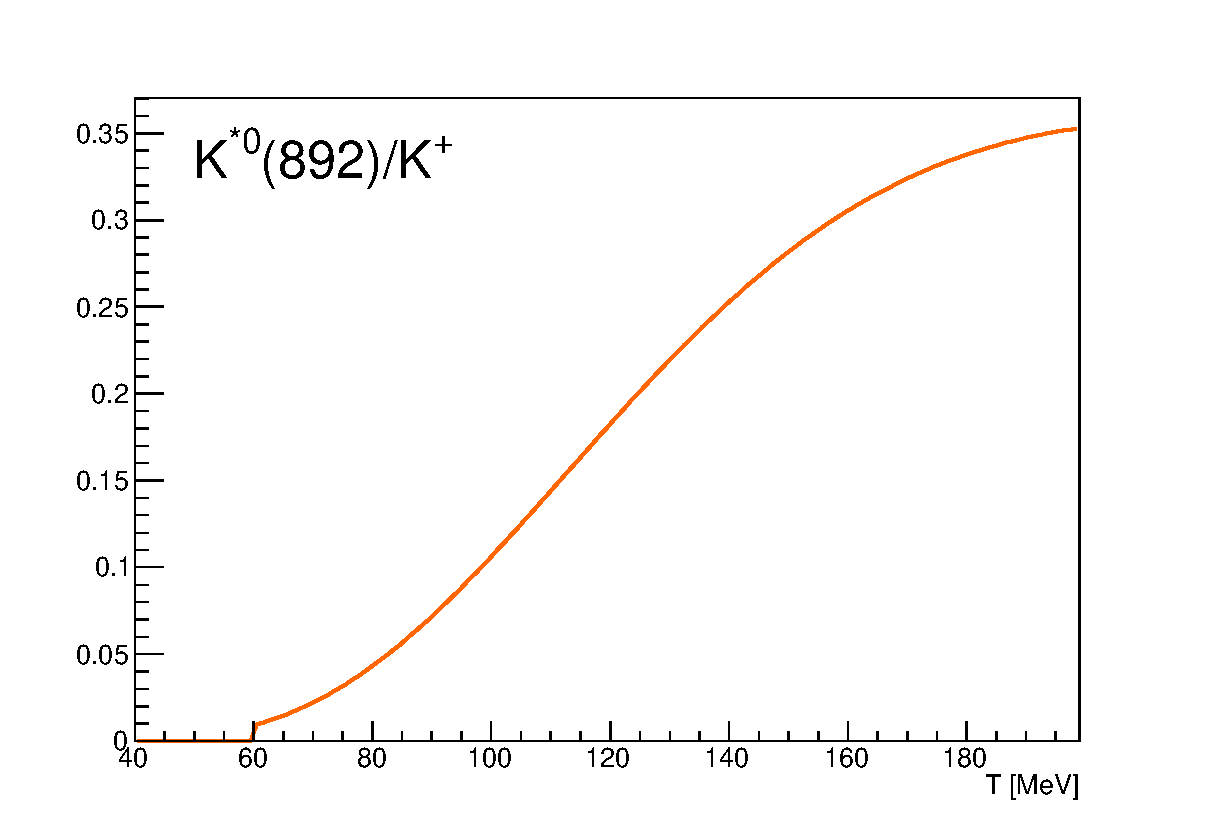
\includegraphics[width=200px]{./Version1/FigChapter3/KStarToK}
       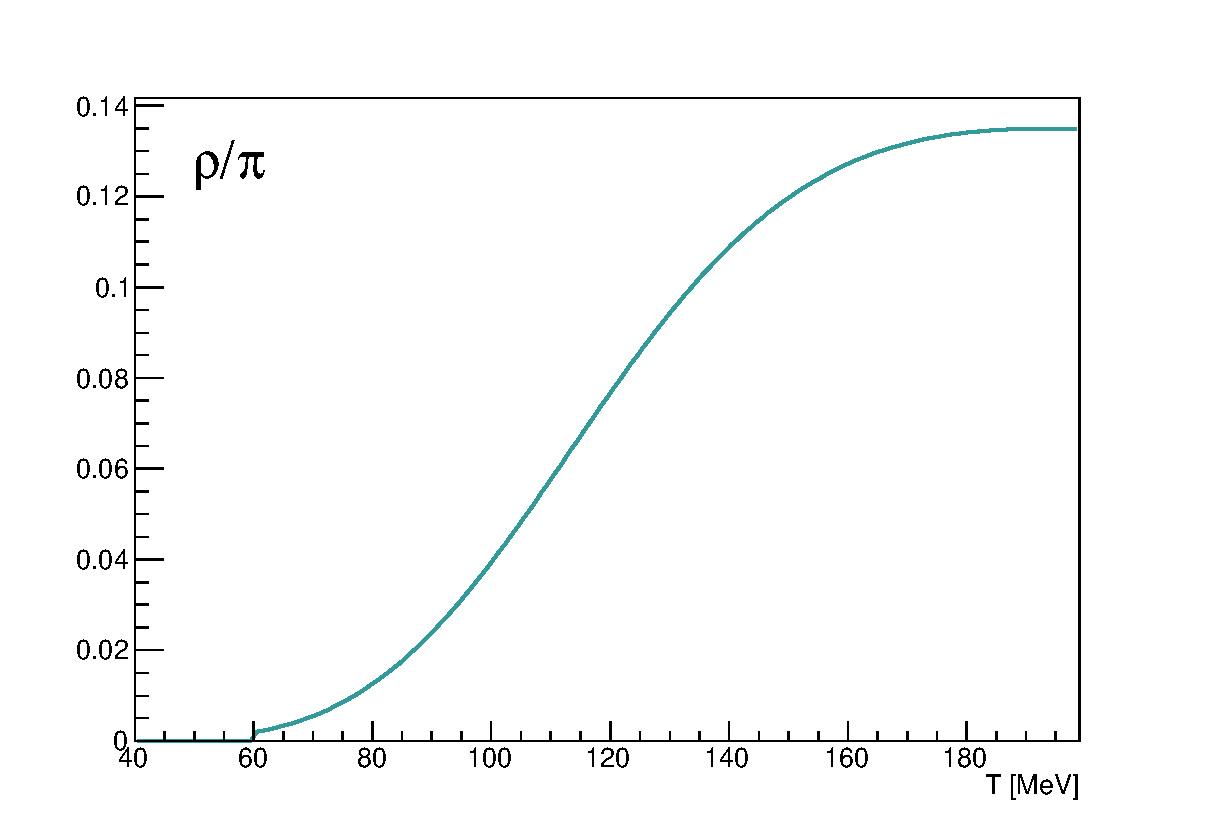
\includegraphics[width=200px]{./Version1/FigChapter3/RhoToPion}
        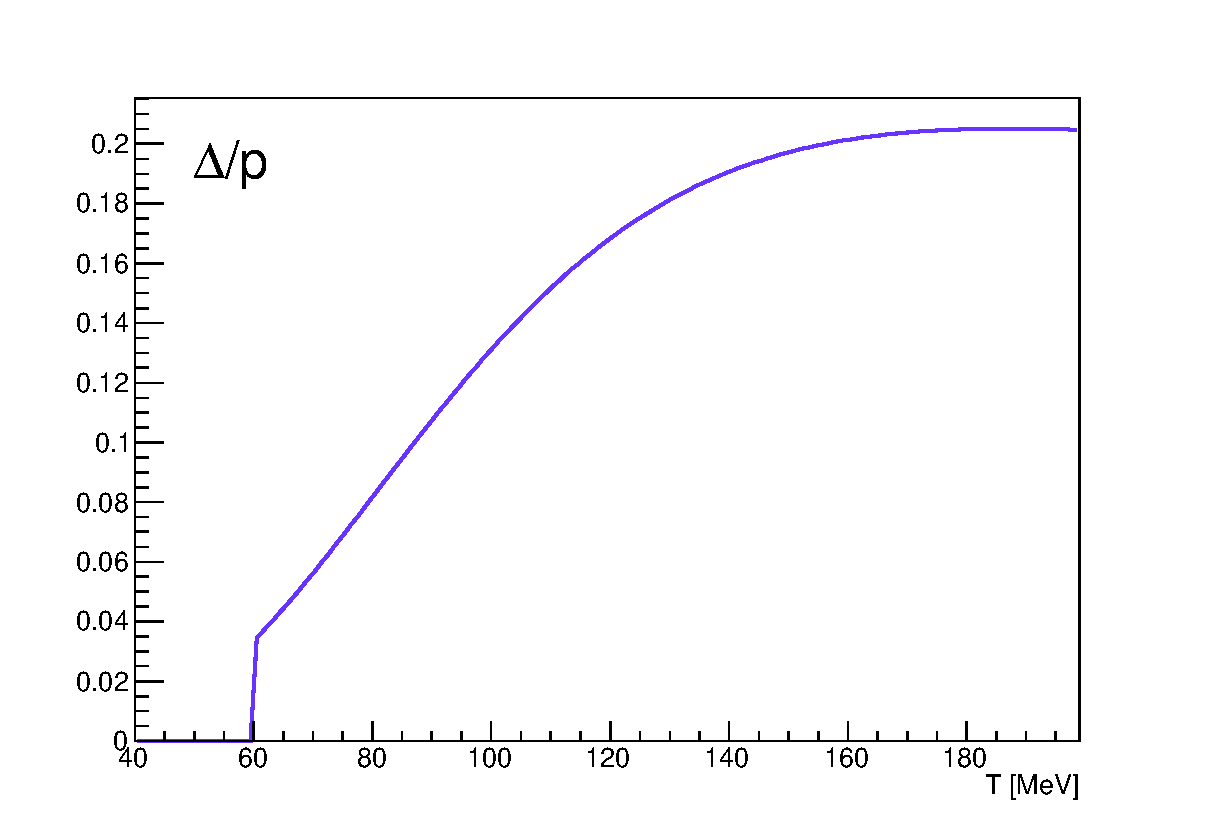
\includegraphics[width=200px]{./Version1/FigChapter3/DeltaToProton}
		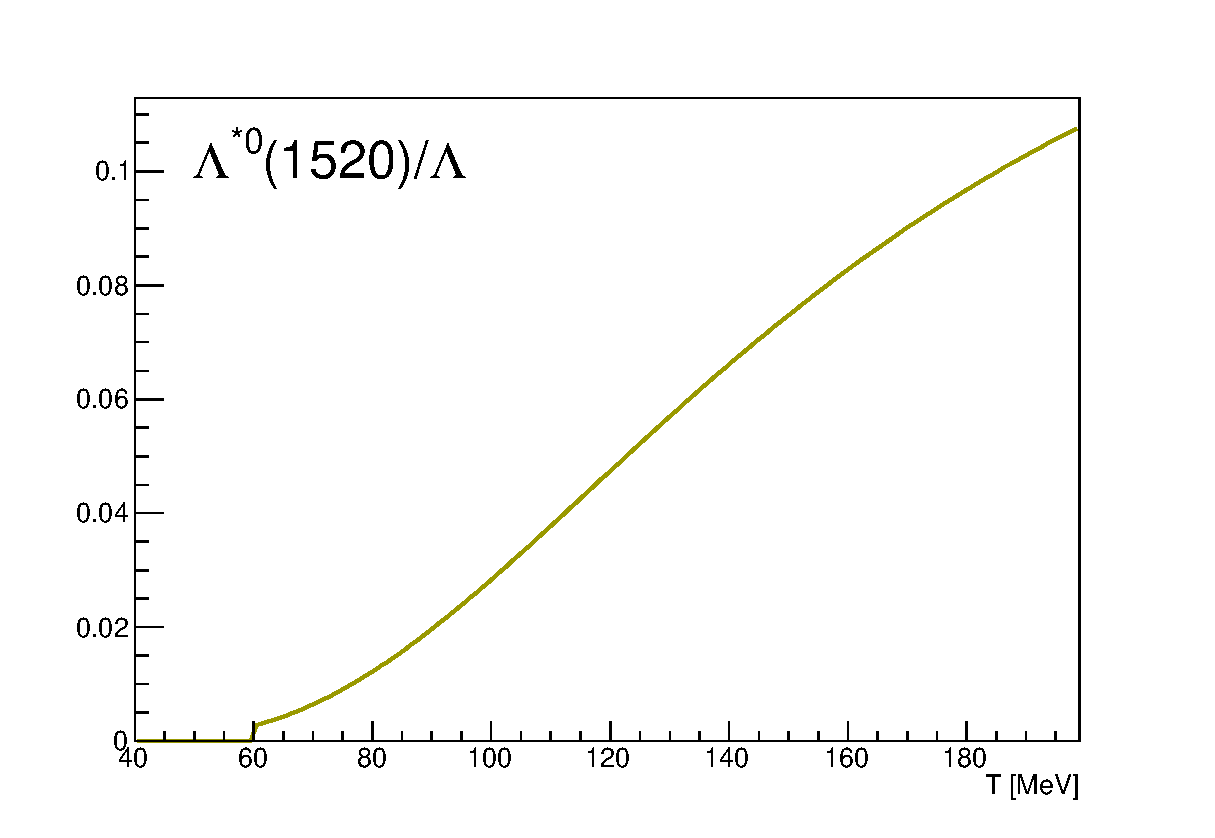
\includegraphics[width=200px]{./Version1/FigChapter3/LambdaStarToLambda}
		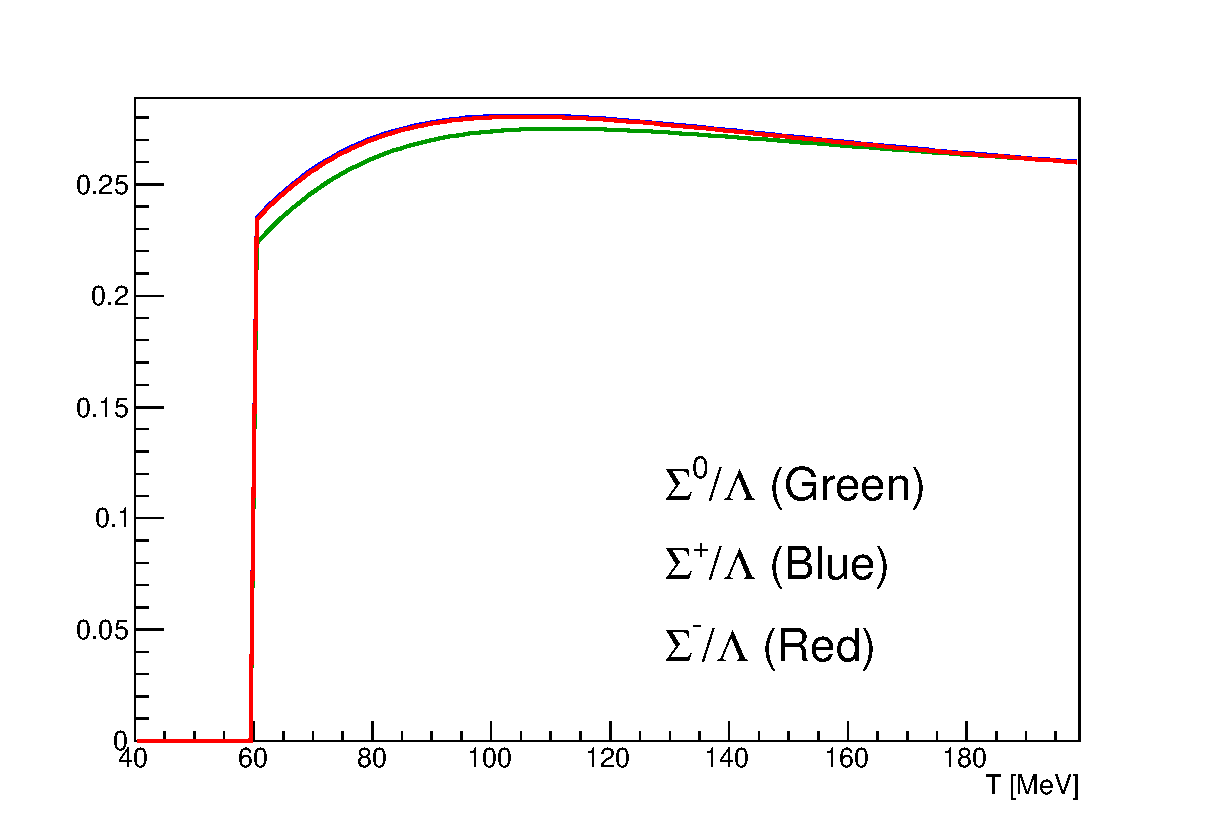
\includegraphics[width=200px]{./Version1/FigChapter3/SigmaRatio}
		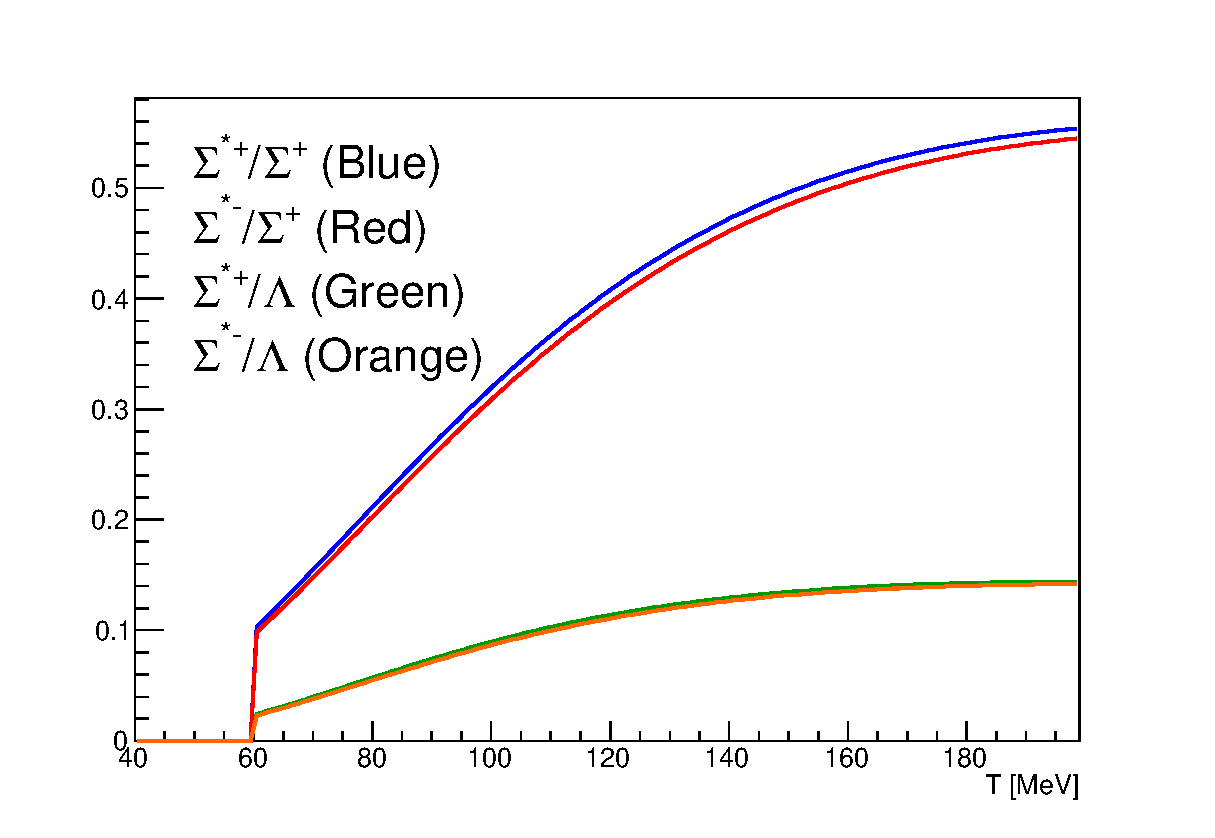
\includegraphics[width=200px]{./Version1/FigChapter3/SigmaStarRatio}
		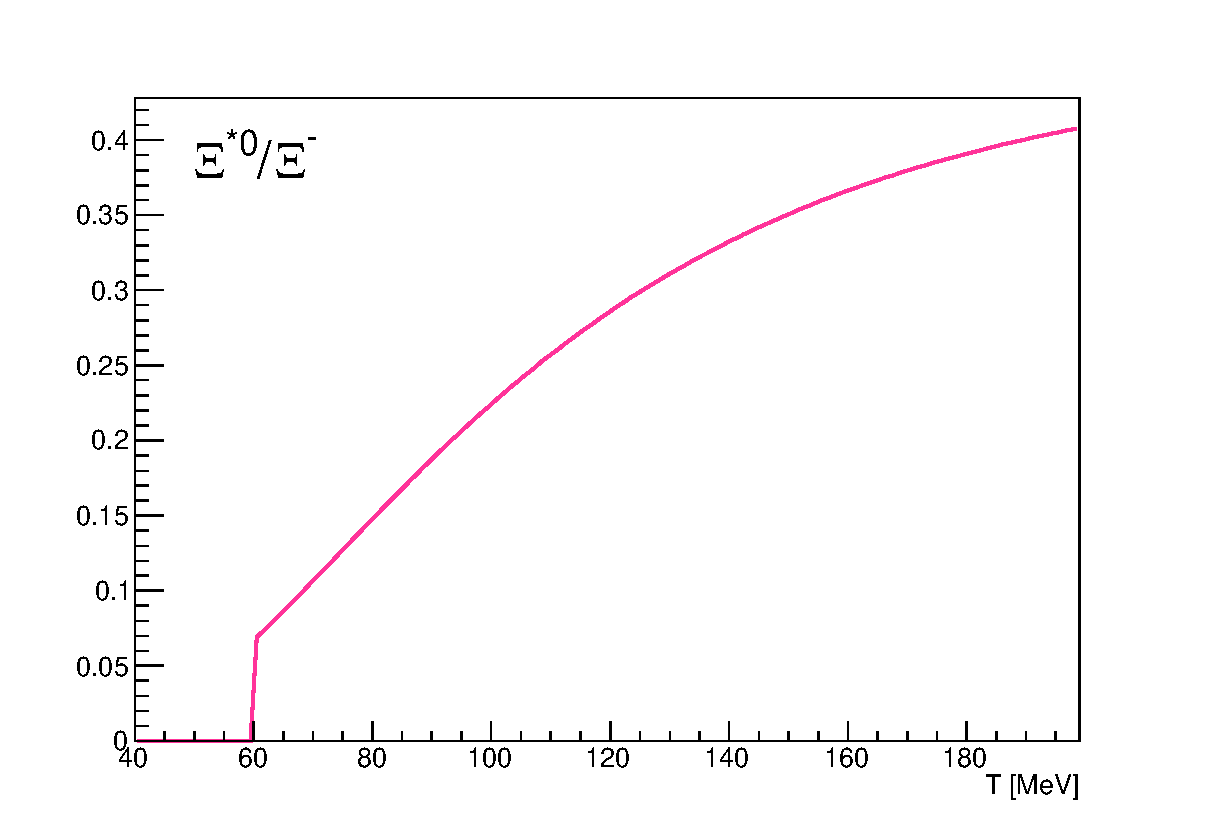
\includegraphics[width=200px]{./Version1/FigChapter3/XiStarToXi}
		\caption{\label{result1} Ratio of baryonic and mesonic resonances over their stable partner as a function of temperature.}
	\end{center}\hspace{2pc}%
\end{figure}

\newpage

\subsubsection{Comparison with data}

\begin{figure}[!htbp]
\begin{center}
	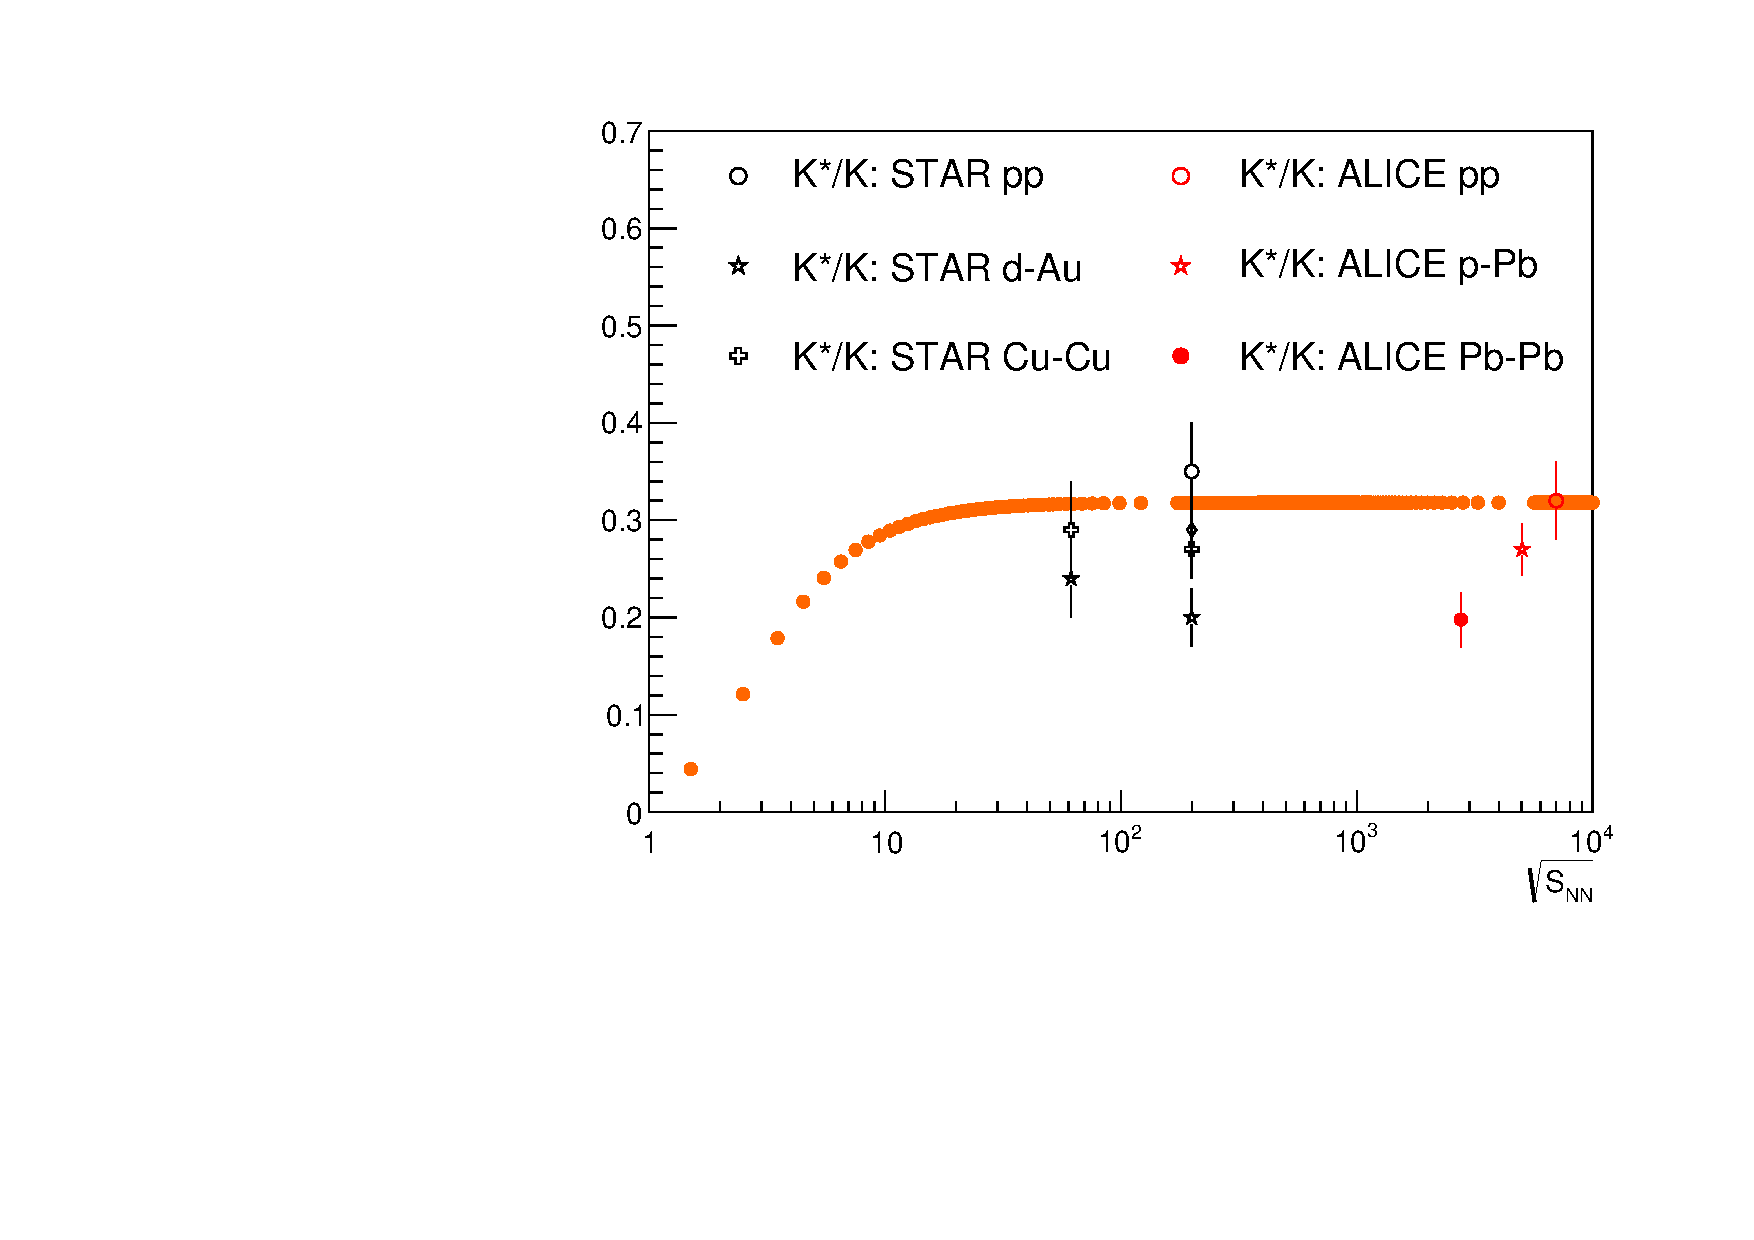
\includegraphics[width=200px]{./Version1/FigChapter3/Kstar_sqrt_s.pdf}
	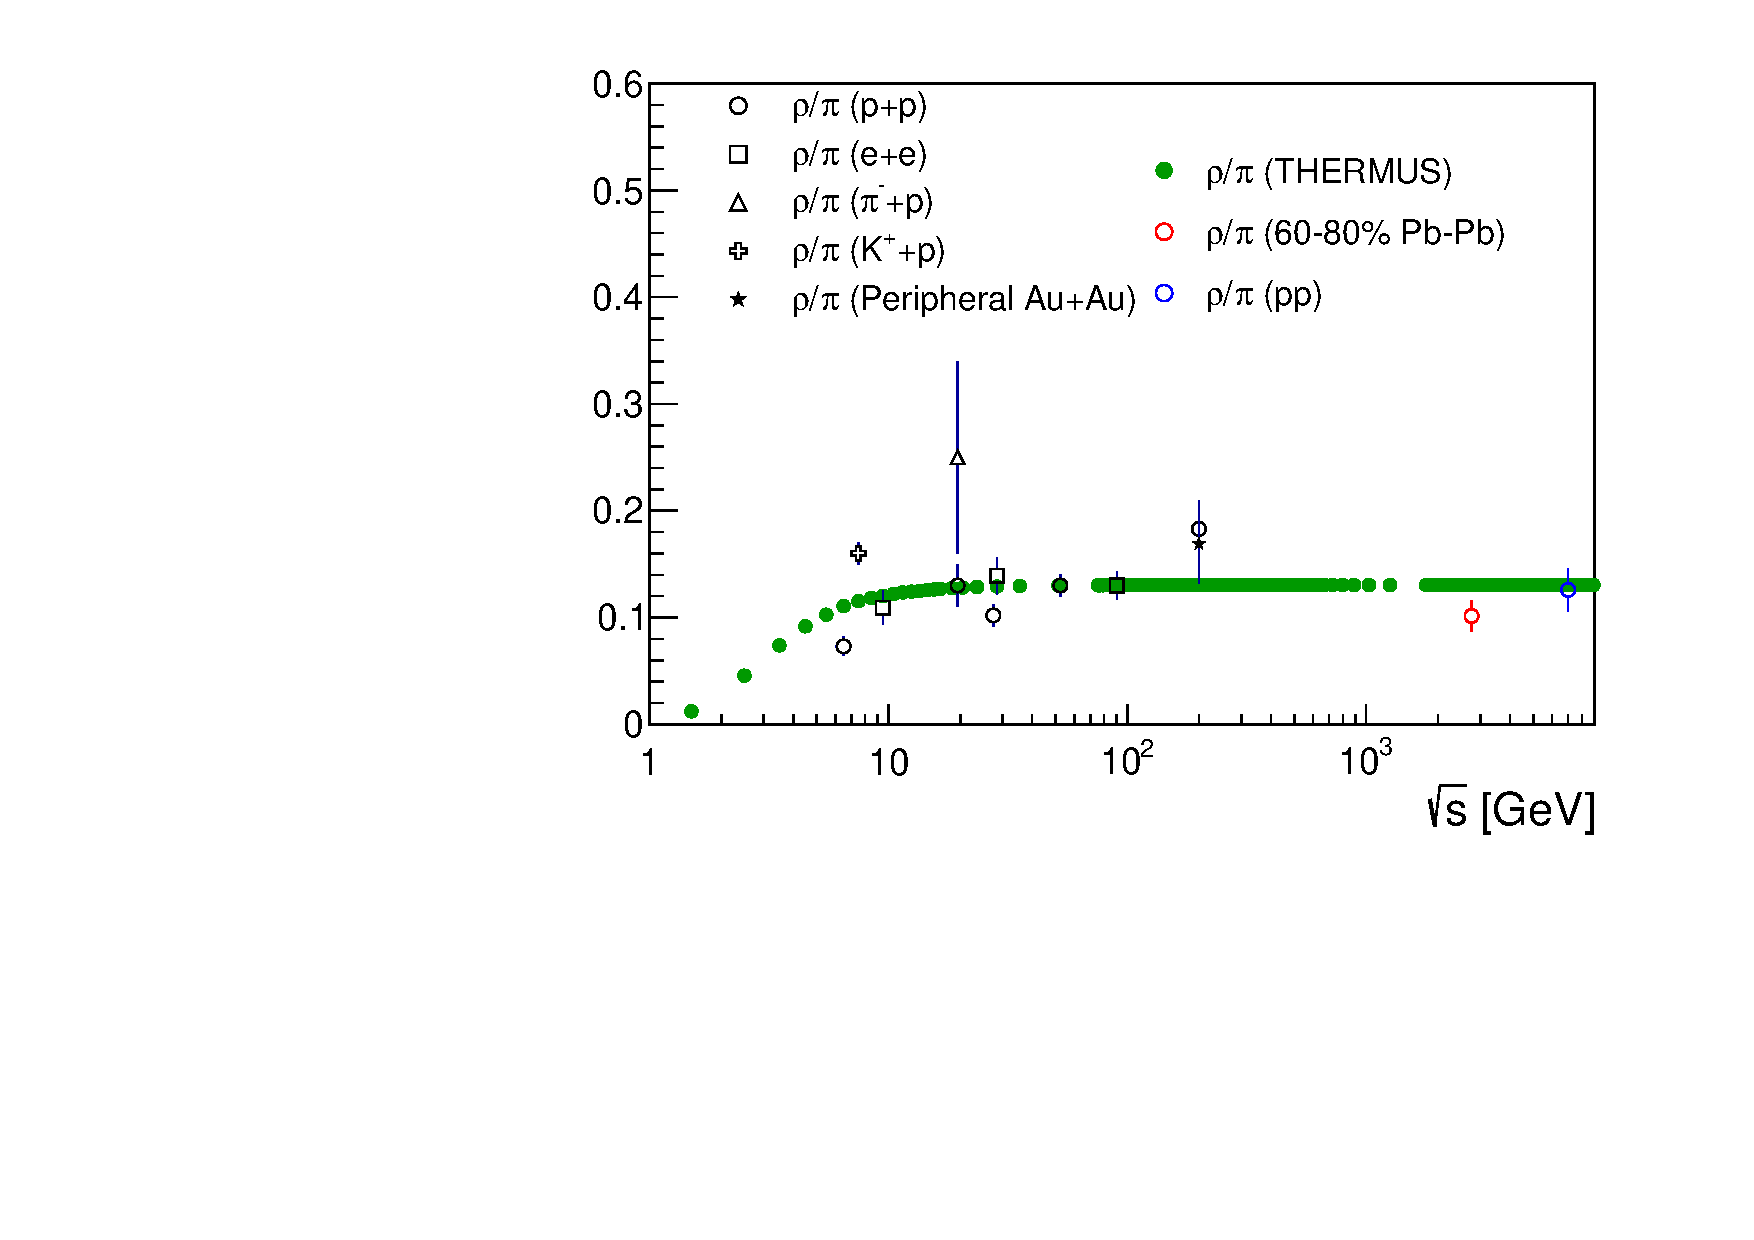
\includegraphics[width=200px]{./Version1/FigChapter3/RhoToPion_sqrt_s.pdf}
	\caption{\label{result2} Ratio of resonances over their stable partner as a function of $\sqrt{(s)}$.}
\end{center}\hspace{2pc}%
\end{figure}



\subsection{UrQMD}